%%%%%%%%%%%%%%%%%%%%%%%%%%%%%%%%%%%%%%%%%%%%%%%%%%%%%%%%%%%%%%%%%%%%%%%%%%%%%%%
\chapter{Parte Digitale}
\section{Inverter CMOS e Margini di Rumore}

\subsection{Funzione di trasferimento di un inverter CMOS, definizione e metodologie di calcolo del margine di rumore (Solo scritto)}

Consideriamo il circuito dell'inverter CMOS rappresentato in Figura~\ref{fig:inverter_cmos}.\\[2mm]
\begin{figure}[H]
    \centering
    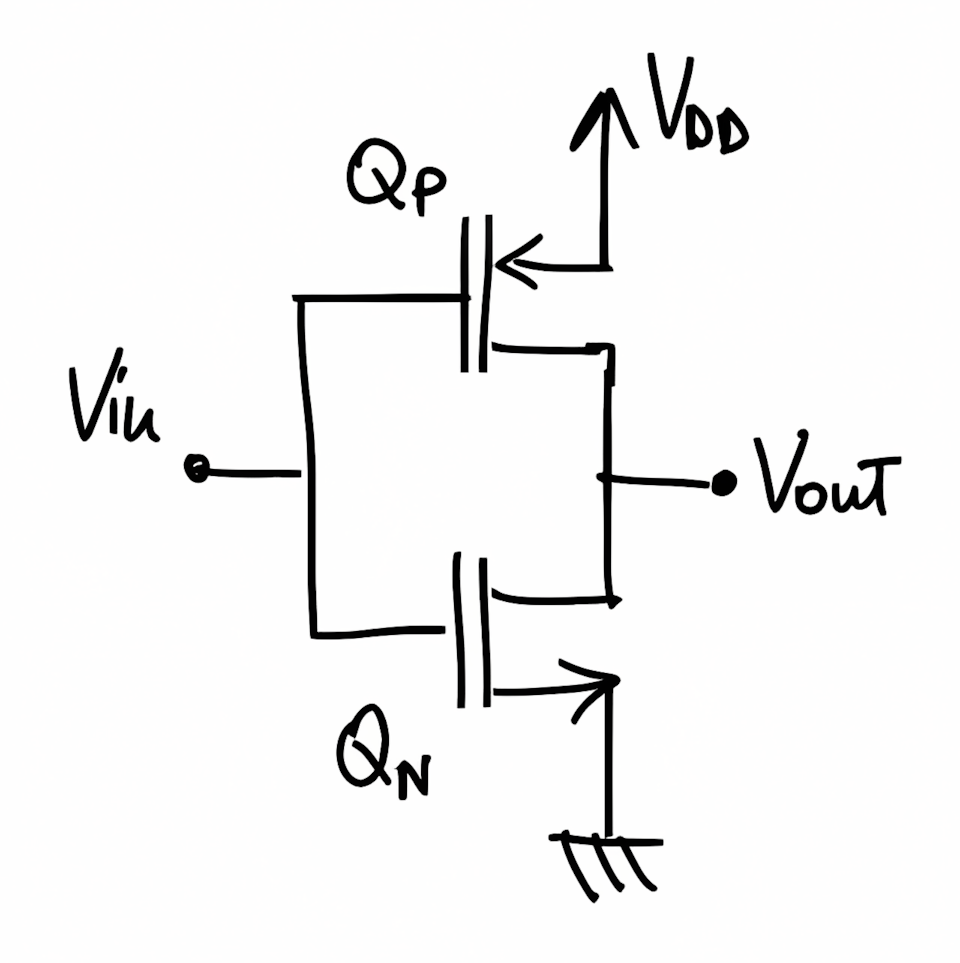
\includegraphics[width=0.6\textwidth]{images/2.1.1.1.png}
    \caption{Inverter CMOS, composto da un transistor PMOS \(Q_P\) e un NMOS \(Q_N\).}
    \label{fig:inverter_cmos}
\end{figure}

Ipotizzando una configurazione simmetrica rispetto a \(V_{DD}/2\) (ovvero \(k_P=k_N\)), la funzione di trasferimento risulta come illustrata in Figura~\ref{fig:funzione_trasferimento}.\\[2mm]
\begin{figure}[H]
    \centering
    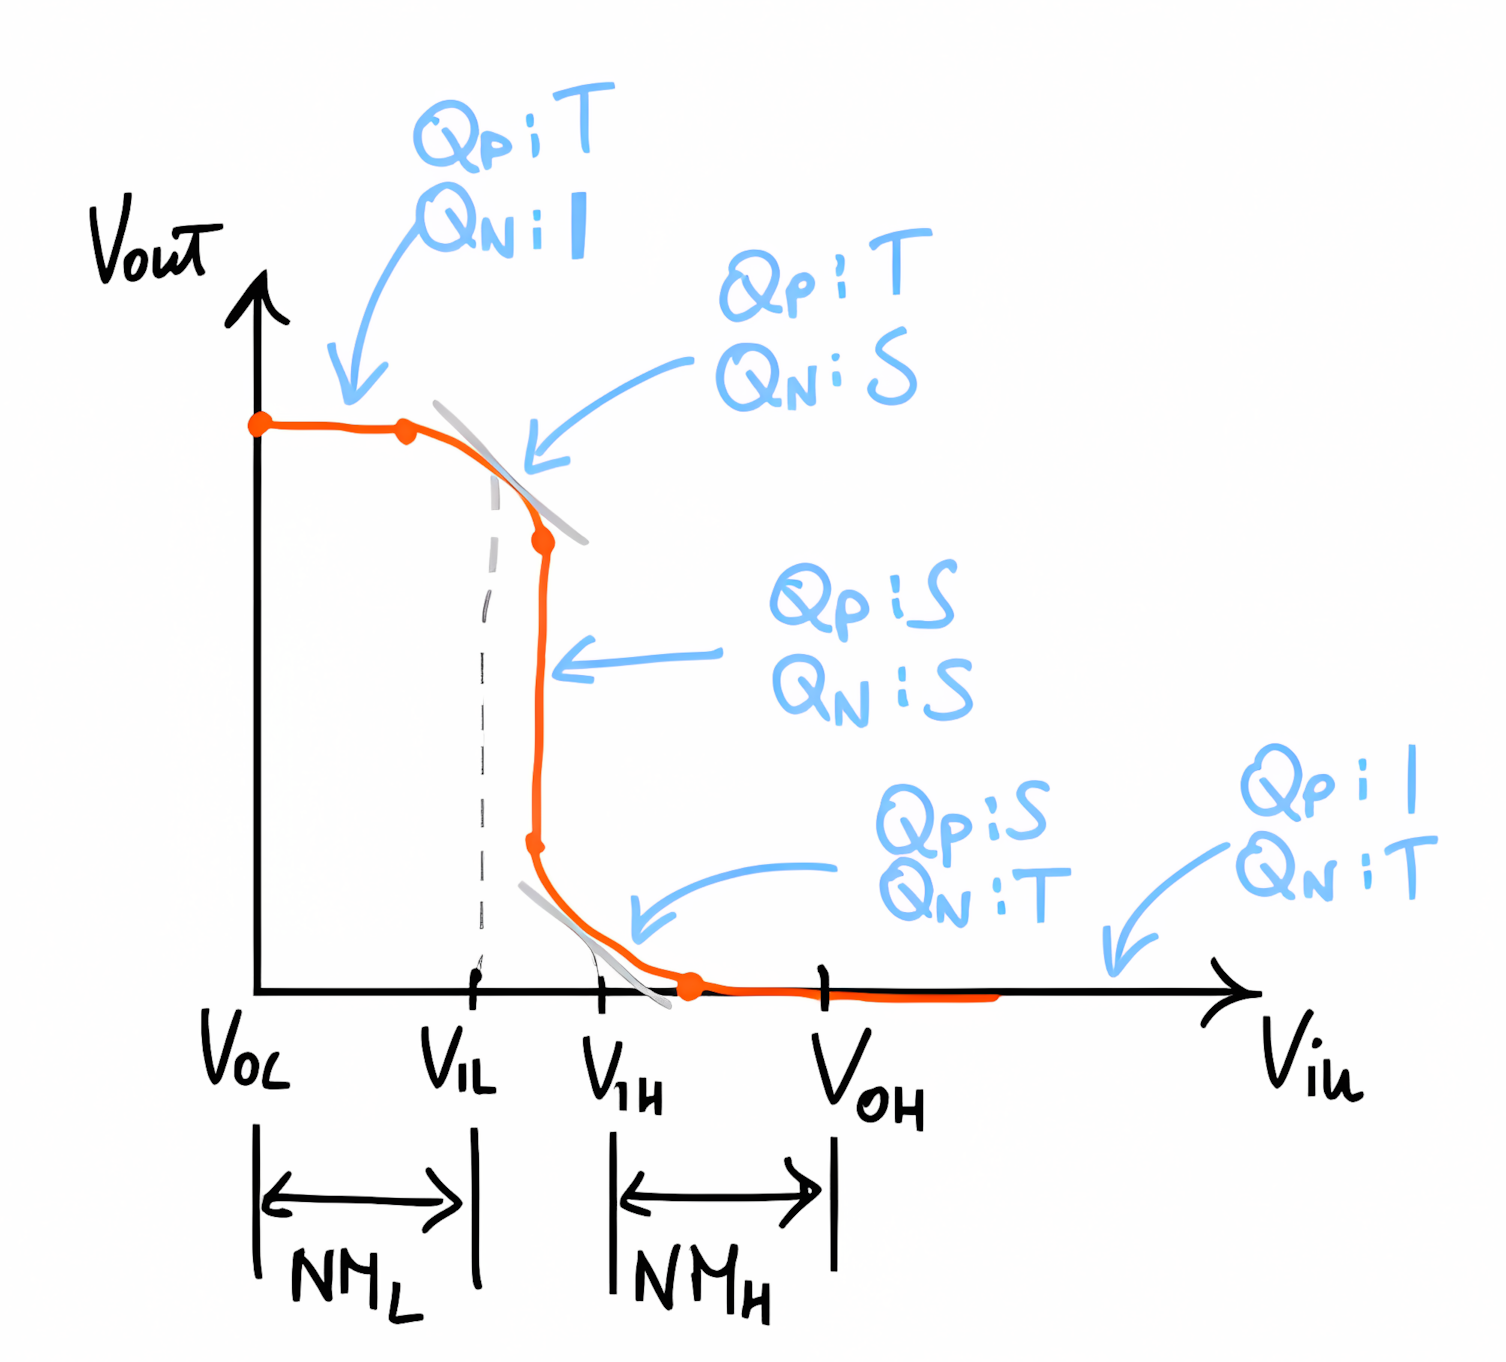
\includegraphics[width=0.6\textwidth]{images/2.1.1.2.png}
    \caption{Funzione di trasferimento dell'inverter CMOS, simmetrica rispetto a \(V_{DD}/2\). Le annotazioni indicano gli stati: ‘I’ = interdizione, ‘T’ = triodo, ‘S’ = saturazione.}
    \label{fig:funzione_trasferimento}
\end{figure}

Il \textbf{margine di rumore} è definito come la variazione massima ammissibile sul segnale d’ingresso, dovuta al rumore, senza che venga alterato l’output. Indichiamo con \(V_{OL}\) e \(V_{OH}\) le tensioni d’uscita per lo stato basso e alto, rispettivamente, e definiamo i valori di soglia \(V_{IL}\) e \(V_{IH}\) come i punti in cui:
\[
\frac{dV_{\text{out}}}{dV_{\text{in}}} = -1.
\]
I margini di rumore sono dunque:
\[
NM_L = V_{IL} - V_{OL}, \quad NM_H = V_{OH} - V_{IH}.
\]

\newpage
\subsection{Disegno del circuito di un inverter logico CMOS e analisi della potenza statica e dinamica}

La potenza dissipata \(P\) si compone di potenza statica \(P_s\) e dinamica \(P_d\):
\[
P = P_s + P_d.
\]
Nel regime statico, in uno stato logico (alto o basso) almeno un transistor è in interdizione, per cui non scorre corrente e \(P_s = V_{DD}\cdot0 = 0\).

Durante la commutazione, invece, le capacità parassite (modellate con un condensatore posto in uscita, vedi Figura~\ref{fig:inverter_potenza}) causano una dissipazione. Il lavoro svolto dal generatore nel passaggio da basso ad alto è:
\[
W_{\text{gen}} = V_{DD}\, Q_c = C\, V_{DD}^2,
\]
con \(Q_c = C V_{DD}\). L'energia immagazzinata nel condensatore è:
\[
E_c = \frac{1}{2}C\, V_{DD}^2.
\]
Quindi, metà dell'energia è immagazzinata e metà dissipata (nel transistor \(Q_P\)). Durante il passaggio da alto a basso, l’energia immagazzinata viene completamente dissipata (nel transistor \(Q_N\)). In un ciclo completo (basso–alto–basso) l'energia totale usata è:
\[
E_{\text{tot}} = C\, V_{DD}^2,
\]
e, considerando una frequenza \(f\), la potenza dinamica risulta:
\[
P_d = f\, C\, V_{DD}^2.
\]
\\[2mm]
\begin{figure}[H]
    \centering
    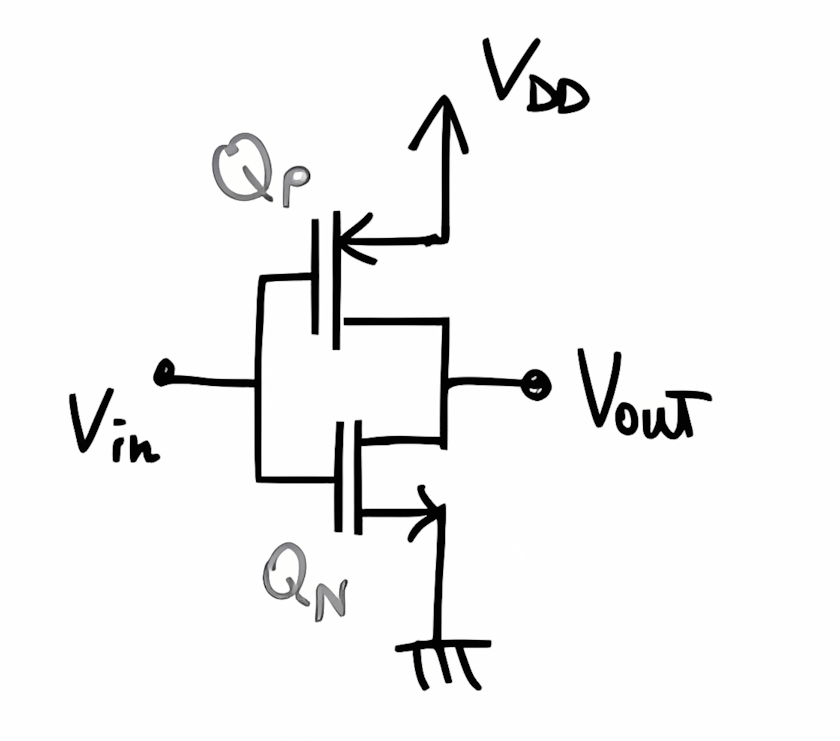
\includegraphics[width=0.8\textwidth]{images/2.1.2.1.png}
    \caption{Struttura di un inverter CMOS.}
    \label{fig:inverter_potenza}
\end{figure}

\\[2mm]
\begin{figure}[H]
    \centering
    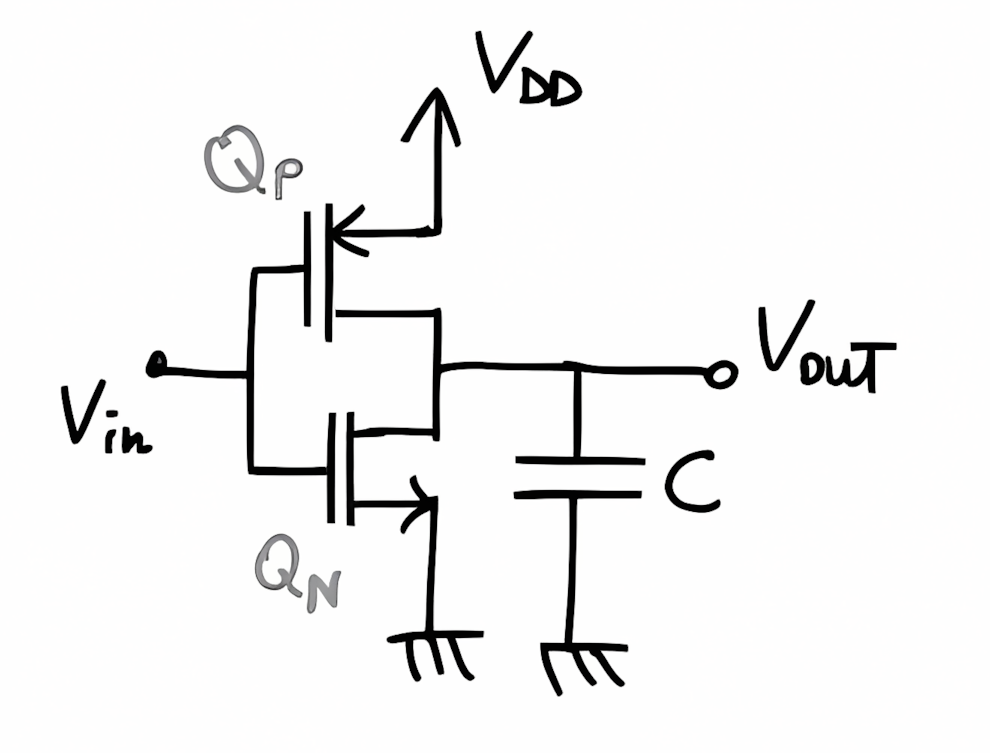
\includegraphics[width=0.8\textwidth]{images/2.1.2.2.png}
    \caption{Struttura equivalente durante la commutazione.}
    \label{fig:inverter_potenza_eq}
\end{figure}

\newpage
\subsection{Funzione di trasferimento ingresso-uscita di un inverter logico CMOS, punti significativi della transcaratteristica e condizioni di simmetria}

La transcaratteristica dell'inverter CMOS è riportata in Figura~\ref{fig:transcaratteristica}.\\[2mm]
\begin{figure}[H]
    \centering
    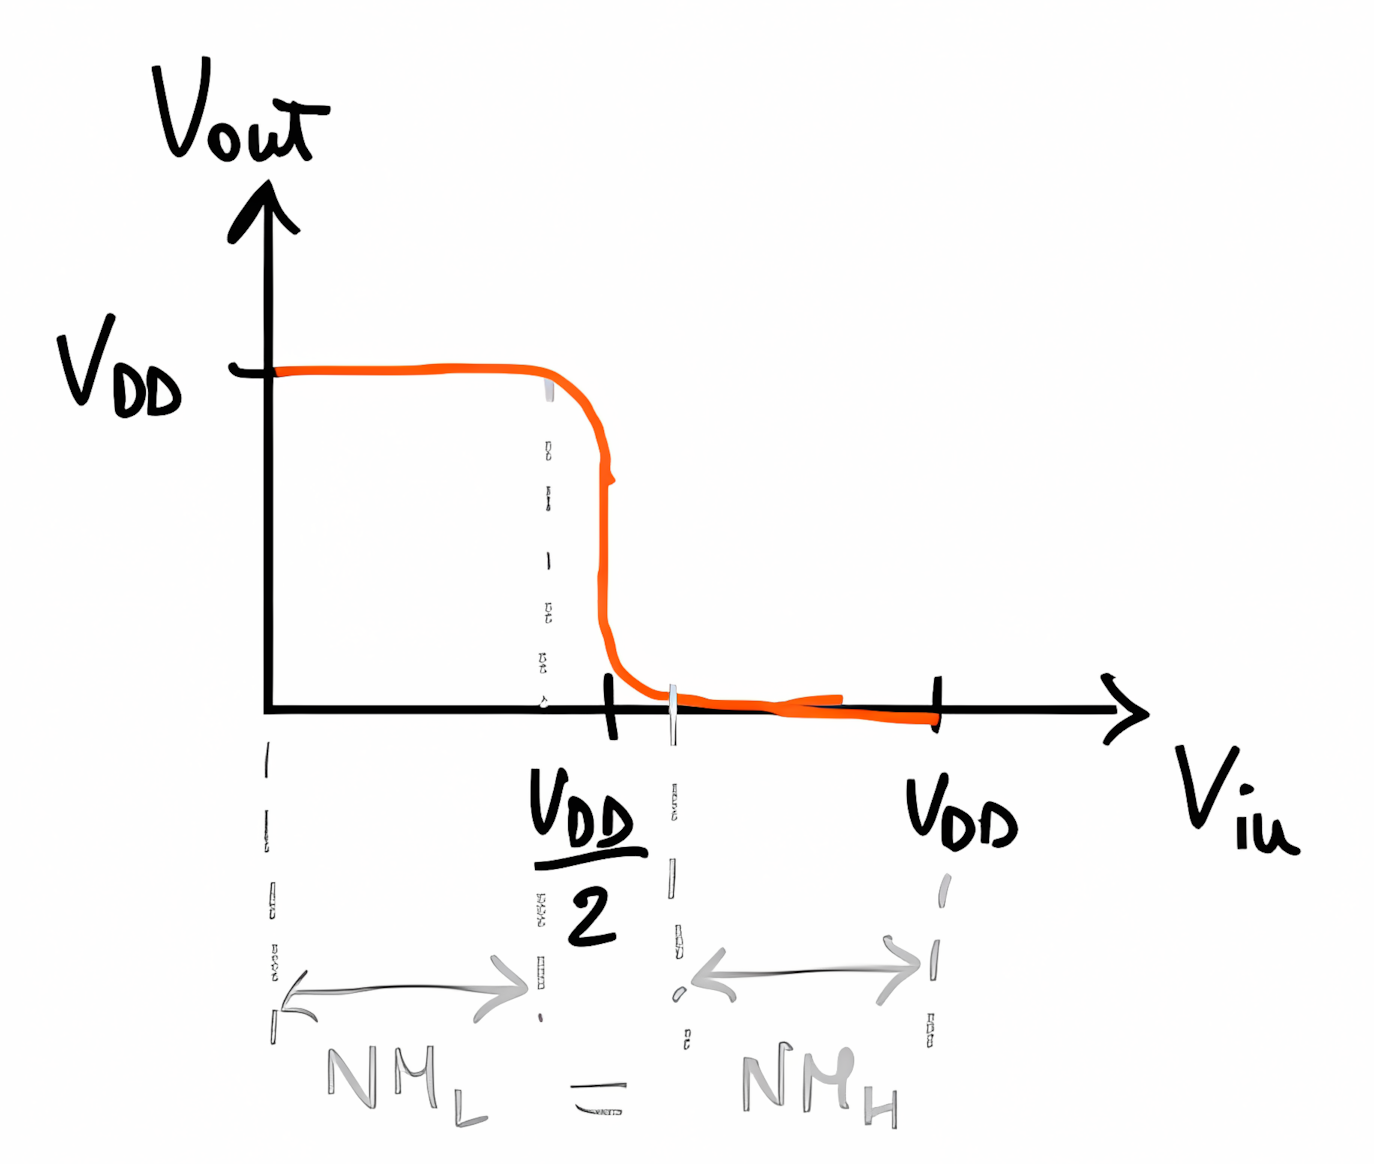
\includegraphics[width=0.6\textwidth]{images/2.1.3.1.png}
    \caption{Transcaratteristica dell'inverter CMOS, simmetrica rispetto a \(V_{DD}/2\).}
    \label{fig:transcaratteristica}
\end{figure}

I punti significativi corrispondono a:
\begin{itemize}
    \item \(V_{\text{in}} = 0\), in cui \(Q_N\) è in interdizione e \(Q_P\) in conduzione (vedi Figura~\ref{fig:transcaratteristica_condizioni}a);
    \item \(V_{\text{in}} = V_{DD}\), dove avviene l'opposto (Figura~\ref{fig:transcaratteristica_condizioni}b);
    \item Il punto in cui entrambi i transistor sono in saturazione, per cui il guadagno (idealmente) è infinito. In condizioni di simmetria questo avviene per \(V_{\text{in}} = V_{DD}/2\).
\end{itemize}

Affinché vi sia simmetria, entrambi i transistor devono essere in saturazione a \(V_{\text{in}} = V_{DD}/2\). Nel CMOS:
\[
V_{GS_N} = V_{\text{in}}, \quad V_{SG_P} = V_{DD} - V_{\text{in}}.
\]
Considerando che in saturazione \(I_N = k_N (V_{GS_N}-V_t)^2\) e \(I_P = k_P (V_{SG_P}-V_t)^2\), e uguagliando le correnti (dato che \(I_P = I_N\)), si ottiene:
\[
k_N (V_{\text{in}}-V_t)^2 = k_P (V_{DD}-V_{\text{in}}-V_t)^2.
\]
Imponendo \(V_{\text{in}} = V_{DD}/2\), si ha:
\[
k_N \left(\frac{V_{DD}}{2}-V_t\right)^2 = k_P \left(\frac{V_{DD}}{2}-V_t\right)^2 \quad \Longrightarrow \quad k_N=k_P.
\]
Pertanto, per avere simmetria è necessario che:
\[
\frac{1}{2} C_{\text{ox}} \mu_N \frac{W_N}{L_N} = \frac{1}{2} C_{\text{ox}} \mu_P \frac{W_P}{L_P} \quad \Longrightarrow \quad \mu_N \frac{W_N}{L_N} = \mu_P \frac{W_P}{L_P}.
\]
Sapendo che la mobilità degli elettroni \( \mu_N \) è circa tre volte quella delle lacune \( \mu_P \), si ottiene:
\[
\frac{W_P}{L_P} \approx 3\, \frac{W_N}{L_N}.
\]
\\[2mm]
\begin{figure}[H]
    \centering
    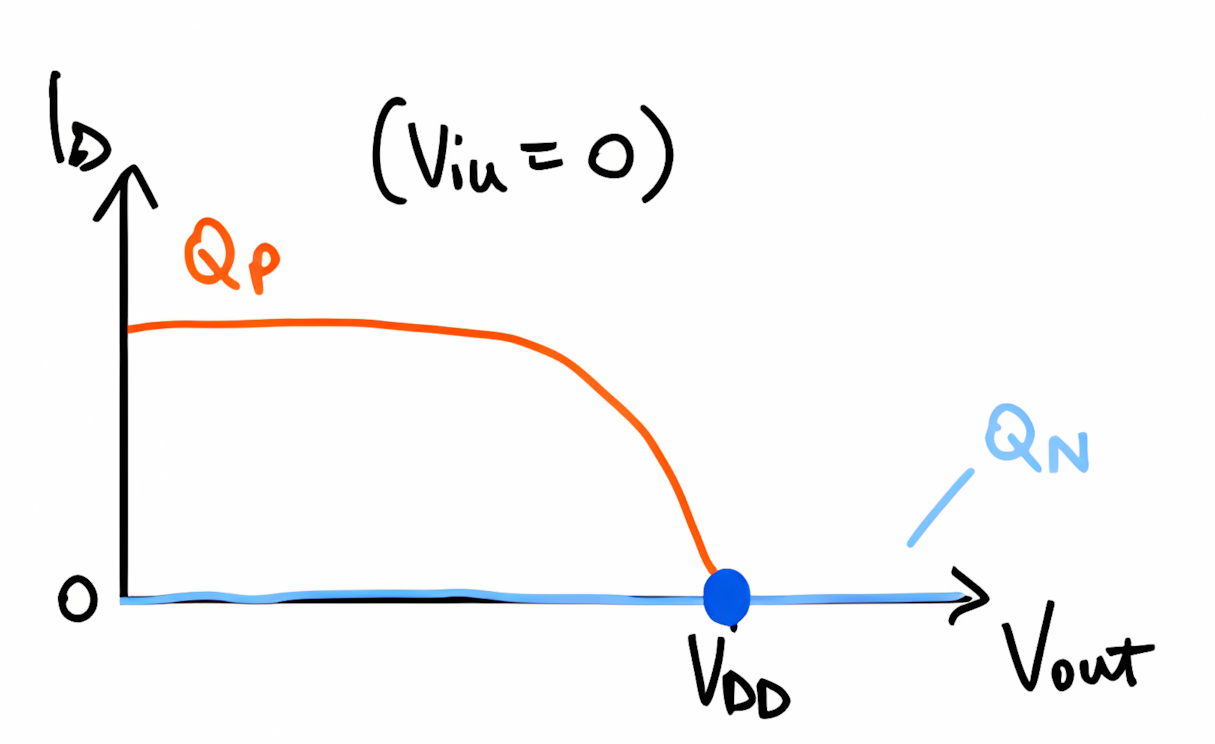
\includegraphics[width=0.6\textwidth]{images/2.1.3.2.png}
    \caption{Curve \(V_{DS_N}\) (azzurro) e \(V_{DD}-V_{SD_P}\) (arancione) in due condizioni: i punti di intersezione sull’asse orizzontale indicano \(V_{\text{out}}\).}
    \label{fig:transcaratteristica_condizioni}
\end{figure}

\newpage
%%%%%%%%%%%%%%%%%%%%%%%%%%%%%%%%%%%%%%%%%%%%%%%%%%%%%%%%%%%%%%%%%%%%%%%%%%%%%%%
\section{Logica e Porte CMOS}

\section{Struttura e funzionamento della NAND e NOR CMOS}
\begin{figure}[H]
  \centering
  \begin{subfigure}[b]{0.45\textwidth}
      \centering
      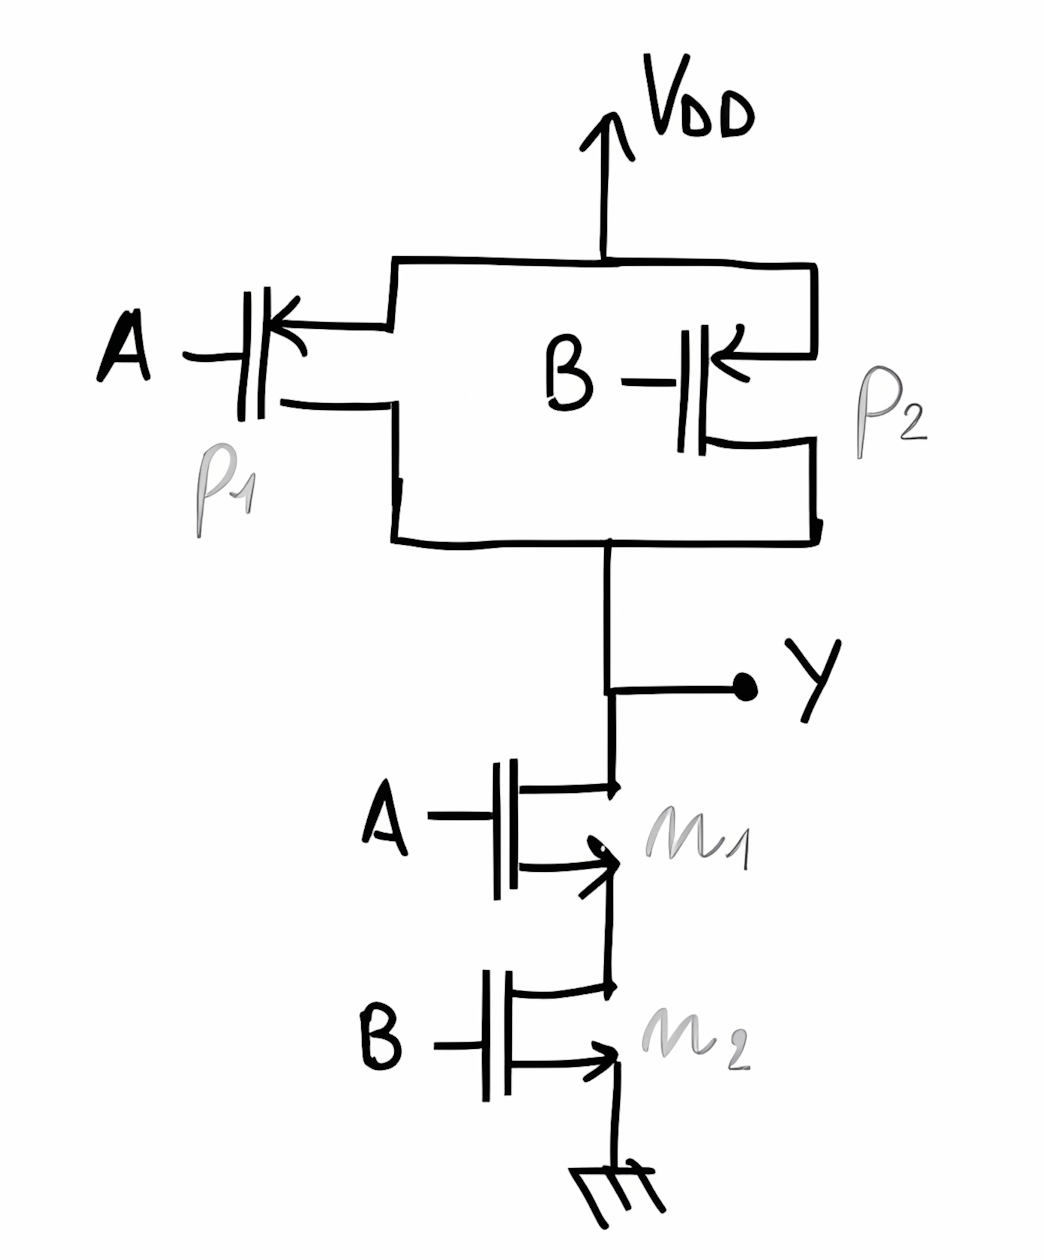
\includegraphics[width=\linewidth]{images/2.2.2.1.png}
      \caption{NAND CMOS}
  \end{subfigure}
  \hfill
  \begin{subfigure}[b]{0.45\textwidth}
      \centering
      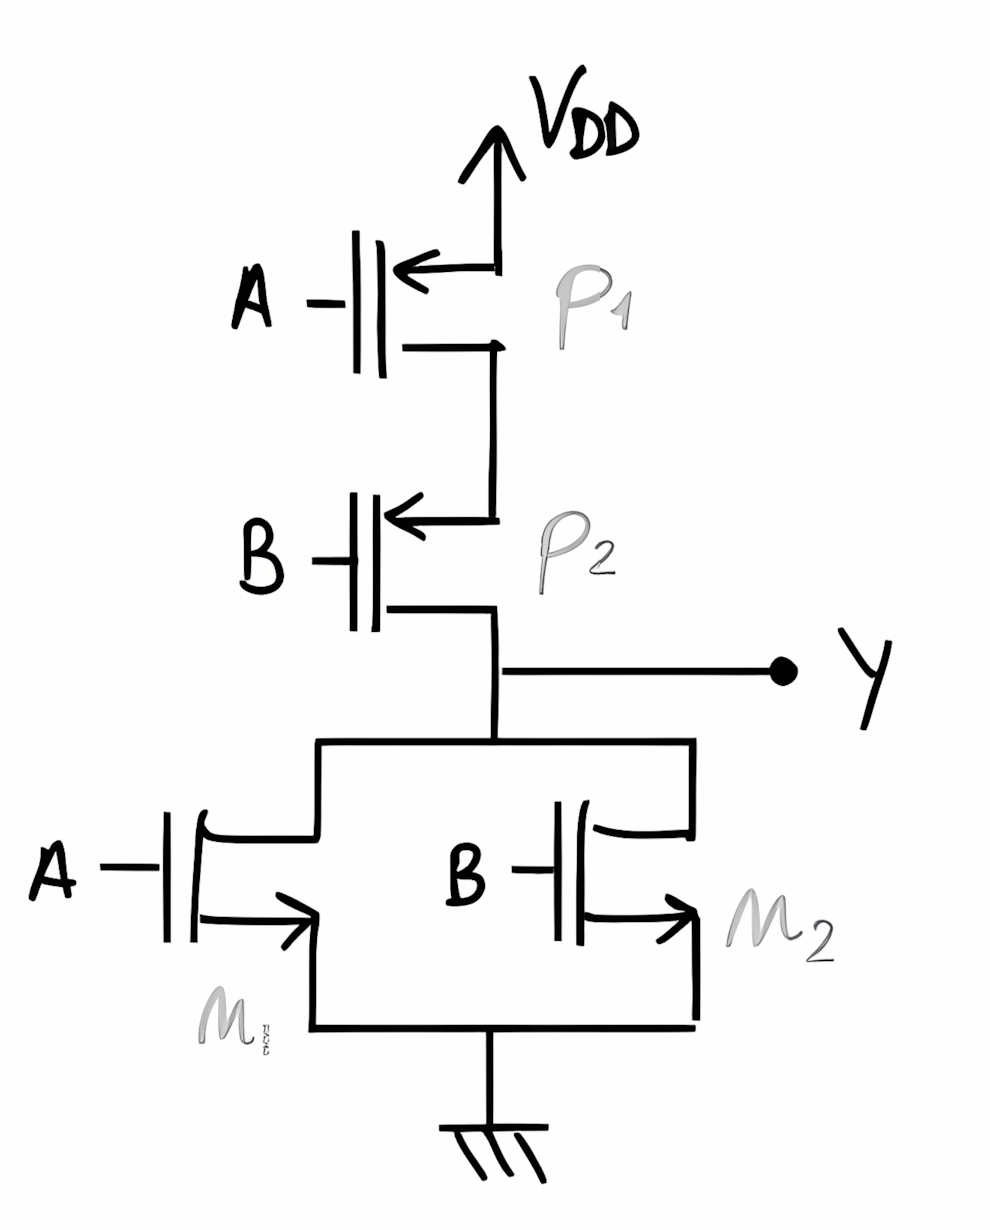
\includegraphics[width=\linewidth]{images/2.2.2.2.png}
      \caption{NOR CMOS}
  \end{subfigure}
  \caption{Figura 30: (a) Schema del circuito NAND CMOS; (b) Schema del circuito NOR CMOS.}
  \label{fig:fig30}
\end{figure}
\subsection{NAND CMOS}
La rete logica NAND implementata con tecnologia CMOS è composta da due sezioni principali:
\begin{enumerate}
  \item \textbf{Rete di pull-up}: Include due PMOS connessi in parallelo.
  \item \textbf{Rete di pull-down}: Composta da due NMOS in serie.
\end{enumerate}

Un vantaggio fondamentale dell'architettura CMOS è che, indipendentemente dalla combinazione logica degli ingressi \(A\) e \(B\), non si verifica mai un collegamento diretto tra \(V_{DD}\) e massa. In questo modo si elimina la dissipazione di potenza statica, perché non c'è un percorso continuo per la corrente in condizioni statiche.

\bigskip
\textbf{Funzionamento:}
\begin{itemize}
  \item Se almeno uno degli ingressi è basso, almeno uno dei PMOS risulta in conduzione, dato che in tali condizioni la tensione al loro terminale source-gate è \(V_{SG}=V_{DD}\) (che supera la soglia \(V_t\)). Nel contempo, nella rete di pull-down, almeno uno degli NMOS è interdetto. Di conseguenza l'uscita viene portata a un livello alto, cioè \(V_Y = V_{DD}\).
  \item Quando entrambi gli ingressi sono alti, entrambi i PMOS sono interdetti mentre i NMOS, collegati in serie, conducono. In questo caso, l'uscita viene collegata a massa, cioè \(V_Y = 0\).
\end{itemize}

\subsection{NOR CMOS}

La struttura del NOR CMOS è sostanzialmente opposta a quella del NAND:
\begin{enumerate}
  \item \textbf{Rete di pull-up}: Include due PMOS connessi in serie.
  \item \textbf{Rete di pull-down}: Composta da due NMOS connessi in parallelo.
\end{enumerate}

\bigskip
\textbf{Funzionamento:}
\begin{itemize}
  \item Se entrambi gli ingressi sono bassi, entrambi i PMOS sono in conduzione (poiché \(V_{SG}=V_{DD}>V_t\)) e gli NMOS sono interdetti. In questo caso l'uscita è portata a un livello alto, cioè \(V_Y = V_{DD}\).
  \item Se almeno uno degli ingressi è alto, almeno uno dei PMOS è interdetto, mentre nella rete di pull-down almeno uno degli NMOS conduce. Di conseguenza, l'uscita viene collegata a massa, ovvero \(V_Y = 0\).
\end{itemize}

\subsection*{Figura 30}

\textbf{(a)} \textit{Circuito NAND CMOS}: La rete di pull-up è formata dai PMOS \(P_1\) e \(P_2\) in parallelo, mentre la rete di pull-down include gli NMOS \(M_1\) e \(M_2\) connessi in serie.

\bigskip

\textbf{(b)} \textit{Circuito NOR CMOS}: La rete di pull-up è composta da \(P_1\) e \(P_2\) in serie, mentre la rete di pull-down è costituita da \(M_1\) e \(M_2\) in parallelo.

\subsection{Porta NOR con tasso di occupazione d’area (Solo scritto)}
% Contenuto da integrare in futuro.
\bigskip

\newpage

%%%%%%%%%%%%%%%%%%%%%%%%%%%%%%%%%%%%%%%%%%%%%%%%%%%%%%%%%%%%%%%%%%%%%%%%%%%%%%%
\section{Tempi di Ritardo}

\subsection{I tempi di ritardo alto-basso e basso-alto}

Considerando un inverter logico, il tempo di ritardo è definito come l’intervallo tra il momento in cui l’ingresso \(v_{\text{in}}\) raggiunge il 50\% del valore finale e quello in cui l’uscita raggiunge il 50\% del relativo valore finale. Se l’uscita passa da alto a basso, il tempo è denominato \emph{tempo di ritardo alto-basso} \(t_{\text{PHL}}\), mentre se passa da basso ad alto si parla di \emph{tempo di ritardo basso-alto} \(t_{\text{PLH}}\). La media di questi due tempi definisce il tempo di propagazione:
\[
t_p = \frac{t_{\text{PHL}} + t_{\text{PLH}}}{2}.
\]
\\[2mm]
\begin{figure}[H]
    \centering
    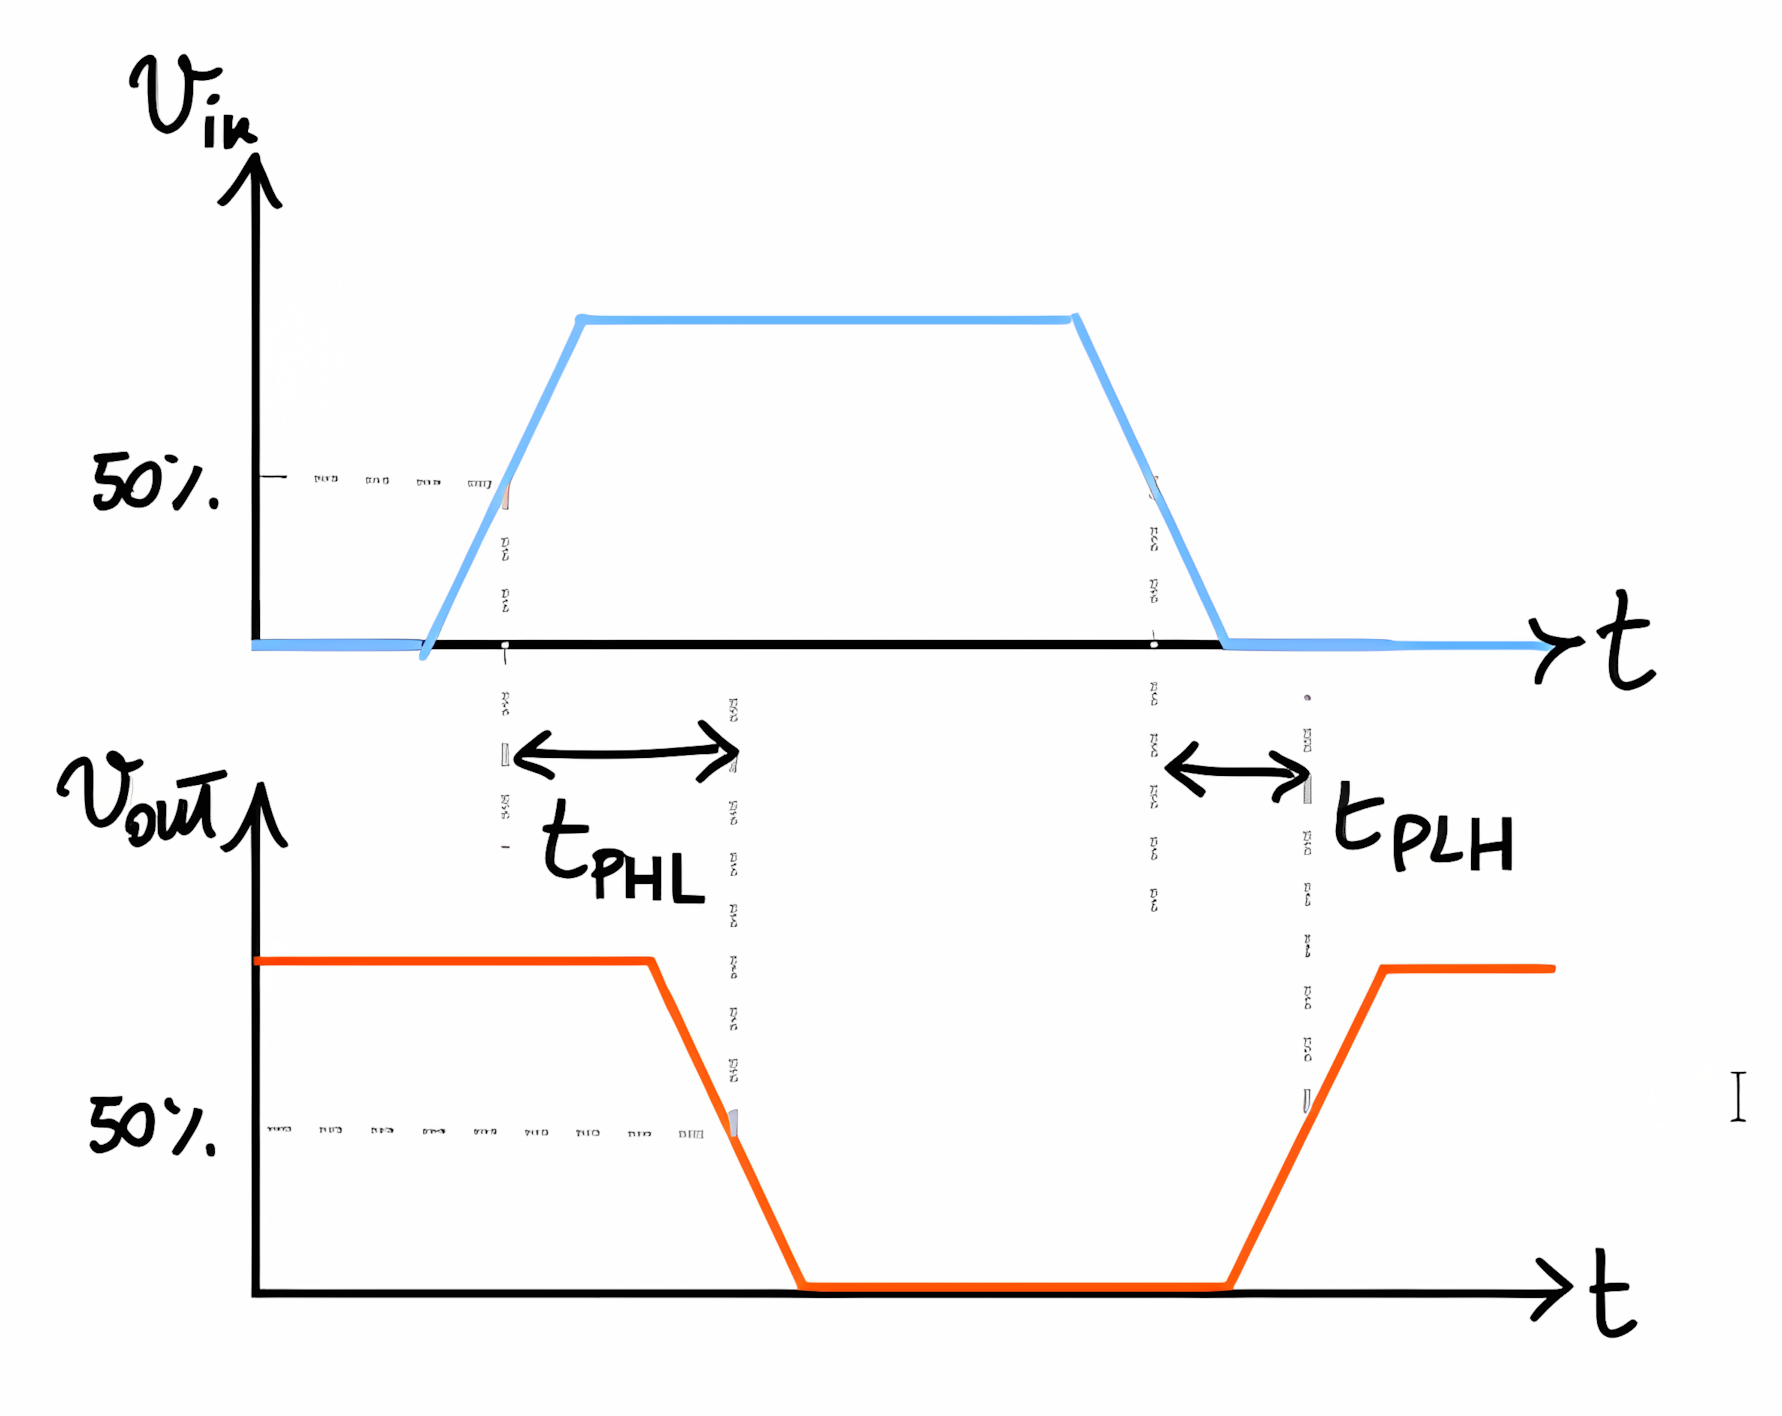
\includegraphics[width=0.6\textwidth]{images/2.3.1.1.png}
    \caption{Diagramma dei tempi di ritardo: si considerano i tempi in uscita.}
    \label{fig:tempi_ritardo}
\end{figure}

\newpage
%%%%%%%%%%%%%%%%%%%%%%%%%%%%%%%%%%%%%%%%%%%%%%%%%%%%%%%%%%%%%%%%%%%%%%%%%%%%%%%
\section{Altri Amplificatori e Argomenti Digitali}

\subsection{Inverter NMOS}
Nella tecnologia NMOS il circuito è come mostrato in Figura~\ref{fig:NMOS_inverter}. Per calcolare i margini di errore, occorre innanzitutto derivare analiticamente la funzione di trasferimento e poi calcolare la derivata, imponendola pari a \(-1\). Questa condizione identifica il punto centrale della zona di utilità del transistor come amplificatore, mentre le regioni a destra e a sinistra corrispondono ai margini di errore nei circuiti digitali.

Nel circuito, due transistor \(Q_1\) e \(Q_2\) sono collegati in serie, per cui, in analisi statica (dove il condensatore che modella le capacità parassite è considerato circuito aperto), si impone la condizione
\[
I_{D1} = I_{D2}.
\]
La corrente di drain di \(Q_1\), che opera in saturazione, è data da
\[
I_{D1} = K_1\,(V_{GS1} - V_{TN1})^2,
\]
mentre la corrente di drain di \(Q_2\), operante in triodo, è espressa da
\[
I_{D2} = K_2\,\Bigl[(V_{GS2} - V_{TN2})\,V_{DS2} - V_{DS2}^2\Bigr].
\]
Uguagliando le due correnti si ottiene l'equazione:
\[
K_1\,(V_{IN} - V_{TN1})^2 = K_2\Bigl[(0 - V_{IN})(V_{DD}-V_{OUT}) - (V_{DD}-V_{OUT})^2\Bigr].
\]
Questa equazione rappresenta la funzione di trasferimento \(V_{OUT}=f(V_{IN})\). Calcolando la derivata di \(f(V_{IN})\) e imponendola pari a \(-1\),
\[
\frac{dV_{OUT}}{dV_{IN}} = -1,
\]
si individuano i due punti che delimitano la zona in cui il transistor opera come amplificatore, ovvero la zona di non determinazione nei circuiti digitali, mentre ai lati di questa zona si trovano i margini di errore.

Un ulteriore problema della tecnologia NMOS riguarda la potenza dissipata. Quando l’ingresso è basso e l’uscita alta, \(Q_1\) è interdetto e \(Q_2\) opera in triodo, per cui la corrente \(I_D\) è nulla e la potenza statica è
\[
P_s = V_{DD}\cdot I_D = 0.
\]
Quando, invece, l’ingresso è alto e l’uscita bassa, \(Q_1\) opera in triodo e \(Q_2\) in saturazione, generando una corrente
\[
I_D = K_2\,(V_{GS2} - V_{TN2})^2 \approx K_2\,V_{DD}^2.
\]
In questo caso la potenza statica dissipata risulta:
\[
P_s = V_{DD}\,K_2\,V_{DD}^2 = K_2\,V_{DD}^3.
\]
Considerando che il circuito trascorre metà del tempo in uno stato e metà nell'altro, la potenza statica media è:
\[
P_{\text{statica}} = \frac{1}{2}\,K_2\,V_{DD}^3.
\]
Infine, la potenza dinamica dovuta alla scarica del condensatore parassita è data da:
\[
P_{\text{dinamica}} = f\,C\,V^2.
\]

\begin{figure}[H]
  \centering
  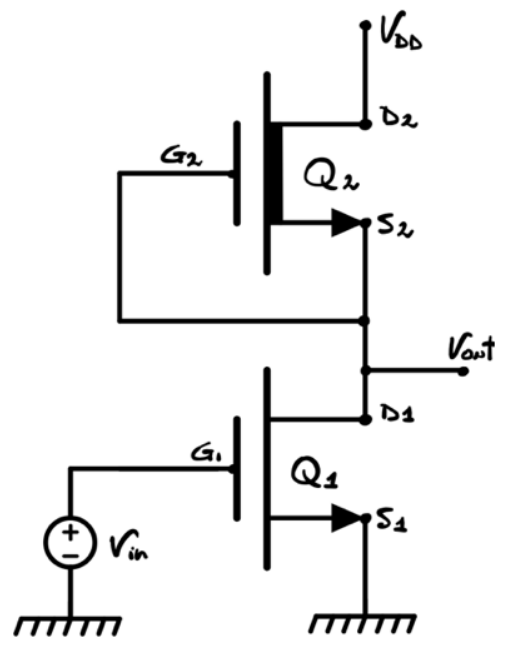
\includegraphics[width=0.8\textwidth]{images/2.5.1.1.png}
  \caption{Inverter in tecnologia NMOS.}
  \label{fig:NMOS_inverter}
\end{figure}
